% ******************************* PhD Thesis Template **************************
% Please have a look at the README.md file for info on how to use the template

\documentclass[a4paper,12pt,times,numbered,print,index]{Classes/PhDThesisPSnPDF}

% ******************************************************************************
% ******************************* Class Options ********************************
% *********************** See README for more details **************************
% ******************************************************************************

% `a4paper'(The University of Cambridge PhD thesis guidelines recommends a page
% size a4 - default option) or `a5paper': A5 Paper size is also allowed as per
% the Cambridge University Engineering Deparment guidelines for PhD thesis
%
% `11pt' or `12pt'(default): Font Size 10pt is NOT recommended by the University
% guidelines
%
% `oneside' or `twoside'(default): Printing double side (twoside) or single
% side.
%
% `print': Use `print' for print version with appropriate margins and page
% layout. Leaving the options field blank will activate Online version.
%
% `index': For index at the end of the thesis
%
% `draftclassic': For draft mode without loading any images (same as draft in book)
%
% `draft': Special draft mode with line numbers, images, and water mark with
% timestamp and custom text. Position of the text can also be modified.
%
% `abstract': To generate only the title page and abstract page with
% dissertation title and name, to submit to the Student Registry
%
% `chapter`: This option enables only the specified chapter and it's references
%  Useful for review and corrections.
%
% ************************* Custom Page Margins ********************************
%
% `custommargin`: Use `custommargin' in options to activate custom page margins,
% which can be defined in the preamble.tex. Custom margin will override
% print/online margin setup.
%
% *********************** Choosing the Fonts in Class Options ******************
%
% `times' : Times font with math support. (The Cambridge University guidelines
% recommend using times)
%
% `fourier': Utopia Font with Fourier Math font (Font has to be installed)
%            It's a free font.
%
% `customfont': Use `customfont' option in the document class and load the
% package in the preamble.tex
%
% default or leave empty: `Latin Modern' font will be loaded.
%
% ********************** Choosing the Bibliography style ***********************
%
% `authoryear': For author-year citation eg., Krishna (2013)
%
% `numbered': (Default Option) For numbered and sorted citation e.g., [1,5,2]
%
% `custombib': Define your own bibliography style in the `preamble.tex' file.
%              `\RequirePackage[square, sort, numbers, authoryear]{natbib}'.
%              This can be also used to load biblatex instead of natbib
%              (See Preamble)
%
% **************************** Choosing the Page Style *************************
%
% `default (leave empty)': For Page Numbers in Header (Left Even, Right Odd) and
% Chapter Name in Header (Right Even) and Section Name (Left Odd). Blank Footer.
%
% `PageStyleI': Chapter Name next & Page Number on Even Side (Left Even).
% Section Name & Page Number in Header on Odd Side (Right Odd). Footer is empty.
%
% `PageStyleII': Chapter Name on Even Side (Left Even) in Header. Section Number
% and Section Name in Header on Odd Side (Right Odd). Page numbering in footer


% ********************************** Preamble **********************************
% Preamble: Contains packages and user-defined commands and settings
% ******************************************************************************
% ****************************** Custom Margin *********************************

% Add `custommargin' in the document class options to use this section
% Set {innerside margin / outerside margin / topmargin / bottom margin}  and
% other page dimensions
\ifsetCustomMargin
  \RequirePackage[left=37mm,right=30mm,top=35mm,bottom=30mm]{geometry}
  \setFancyHdr % To apply fancy header after geometry package is loaded
\fi

% Add spaces between paragraphs
%\setlength{\parskip}{0.5em}
% Ragged bottom avoids extra whitespaces between paragraphs
\raggedbottom
% To remove the excess top spacing for enumeration, list and description
%\usepackage{enumitem}
%\setlist[enumerate,itemize,description]{topsep=0em}

% *****************************************************************************
% ******************* Fonts (like different typewriter fonts etc.)*************

% Add `customfont' in the document class option to use this section

\ifsetCustomFont
  % Set your custom font here and use `customfont' in options. Leave empty to
  % load computer modern font (default LaTeX font).
  %\RequirePackage{helvet}

  % For use with XeLaTeX
  %  \setmainfont[
  %    Path              = ./libertine/opentype/,
  %    Extension         = .otf,
  %    UprightFont = LinLibertine_R,
  %    BoldFont = LinLibertine_RZ, % Linux Libertine O Regular Semibold
  %    ItalicFont = LinLibertine_RI,
  %    BoldItalicFont = LinLibertine_RZI, % Linux Libertine O Regular Semibold Italic
  %  ]
  %  {libertine}
  %  % load font from system font
  %  \newfontfamily\libertinesystemfont{Linux Libertine O}
\fi

% *****************************************************************************
% **************************** Custom Packages ********************************

% ************************* Algorithms and Pseudocode **************************

%\usepackage{algpseudocode}


% ********************Captions and Hyperreferencing / URL **********************

% Captions: This makes captions of figures use a boldfaced small font.
%\RequirePackage[small,bf]{caption}

\RequirePackage[labelsep=space,tableposition=top]{caption}
\renewcommand{\figurename}{Fig.} %to support older versions of captions.sty


% *************************** Graphics and figures *****************************

%\usepackage{rotating}
%\usepackage{wrapfig}

% Uncomment the following two lines to force Latex to place the figure.
% Use [H] when including graphics. Note 'H' instead of 'h'
%\usepackage{float}
%\restylefloat{figure}

% Subcaption package is also available in the sty folder you can use that by
% uncommenting the following line
% This is for people stuck with older versions of texlive
%\usepackage{sty/caption/subcaption}
\usepackage{subcaption}

% ********************************** Tables ************************************
\usepackage{booktabs} % For professional looking tables
\usepackage{multirow}

%\usepackage{multicol}
%\usepackage{longtable}
%\usepackage{tabularx}


% *********************************** SI Units *********************************
\usepackage{siunitx} % use this package module for SI units


% ******************************* Line Spacing *********************************

% Choose linespacing as appropriate. Default is one-half line spacing as per the
% University guidelines

% \doublespacing
% \onehalfspacing
% \singlespacing


% ************************ Formatting / Footnote *******************************

% Don't break enumeration (etc.) across pages in an ugly manner (default 10000)
%\clubpenalty=500
%\widowpenalty=500

%\usepackage[perpage]{footmisc} %Range of footnote options


% *****************************************************************************
% *************************** Bibliography  and References ********************

%\usepackage{cleveref} %Referencing without need to explicitly state fig /table

% Add `custombib' in the document class option to use this section
\ifuseCustomBib
   \RequirePackage[square, sort, numbers, authoryear]{natbib} % CustomBib

% If you would like to use biblatex for your reference management, as opposed to the default `natbibpackage` pass the option `custombib` in the document class. Comment out the previous line to make sure you don't load the natbib package. Uncomment the following lines and specify the location of references.bib file

%\RequirePackage[backend=biber, style=numeric-comp, citestyle=numeric, sorting=nty, natbib=true]{biblatex}
%\bibliography{References/references} %Location of references.bib only for biblatex

\fi

% changes the default name `Bibliography` -> `References'
\renewcommand{\bibname}{References}


% ******************************************************************************
% ************************* User Defined Commands ******************************
% ******************************************************************************

% *********** To change the name of Table of Contents / LOF and LOT ************

%\renewcommand{\contentsname}{My Table of Contents}
%\renewcommand{\listfigurename}{My List of Figures}
%\renewcommand{\listtablename}{My List of Tables}


% ********************** TOC depth and numbering depth *************************

\setcounter{secnumdepth}{2}
\setcounter{tocdepth}{2}


% ******************************* Nomenclature *********************************

% To change the name of the Nomenclature section, uncomment the following line

%\renewcommand{\nomname}{Symbols}


% ********************************* Appendix ***********************************

% The default value of both \appendixtocname and \appendixpagename is `Appendices'. These names can all be changed via:

%\renewcommand{\appendixtocname}{List of appendices}
%\renewcommand{\appendixname}{Appndx}

% *********************** Configure Draft Mode **********************************

% Uncomment to disable figures in `draft'
%\setkeys{Gin}{draft=true}  % set draft to false to enable figures in `draft'

% These options are active only during the draft mode
% Default text is "Draft"
%\SetDraftText{DRAFT}

% Default Watermark location is top. Location (top/bottom)
%\SetDraftWMPosition{bottom}

% Draft Version - default is v1.0
%\SetDraftVersion{v1.1}

% Draft Text grayscale value (should be between 0-black and 1-white)
% Default value is 0.75
%\SetDraftGrayScale{0.8}


% ******************************** Todo Notes **********************************
%% Uncomment the following lines to have todonotes.

%\ifsetDraft
%	\usepackage[colorinlistoftodos]{todonotes}
%	\newcommand{\mynote}[1]{\todo[author=kks32,size=\small,inline,color=green!40]{#1}}
%\else
%	\newcommand{\mynote}[1]{}
%	\newcommand{\listoftodos}{}
%\fi

% Example todo: \mynote{Hey! I have a note}


% ************************ Thesis Information & Meta-data **********************
% Thesis title and author information, refernce file for biblatex
% ************************ Thesis Information & Meta-data **********************
%% The title of the thesis
\title{FscRover}
%\texorpdfstring is used for PDF metadata. Usage:
%\texorpdfstring{LaTeX_Version}{PDF Version (non-latex)} eg.,
%\texorpdfstring{$sigma$}{sigma}

%% Subtitle (Optional)
\subtitle{Rover in F# with coda}

%% The full name of the author
\author{Riccardo Rolla}

%% Department (eg. Department of Engineering, Maths, Physics)
\dept{Dipartimento di Informatica}

%% University and Crest
\university{Università di Pisa}
% Crest minimum should be 30mm.
\crest{
\includegraphics[width=0.2\textwidth]{University_Crest}}
%% Use this crest, if you are using the college crest
%% Crest long miminum should be 65mm
%\crest{
\includegraphics[width=0.45\textwidth]{University_Crest_Long}}

%% College shield [optional] 
% Crest minimum should be 30mm.
%\collegeshield{
\includegraphics[width=0.2\textwidth]{CollegeShields/Kings}}


%% Supervisor (optional)
%% for multiple supervisors, append each supervisor with the \newline command
%\supervisor{\textbf{Prof. A.B. Supervisor\newline
%Prof. C.D. Supervisor\newline
%Prof. E.F. Supervisor\newline
%Prof. G.H. Supervisor}}

%% Supervisor Role (optional) - Supervisor (default) or advisor
% \supervisorrole{\textbf{Supervisors: }}
%% if no title is desired:
% \supervisorrole{}

%% Advisor (optional)
%% for multiple advisors, append each advisor with the \newline command
%\advisor{Advisor 1\newline
%Advisors 2\newline
%Advisor 3\newline
%Advisor 4}
     
%% Advisor Role (optional) - Advisor (default) or leave empty
% \advisorrole{Advisors: }
%% if no title is required
% \advisorrole{}


%% You can redefine the submission text:
% Default as per the University guidelines:
% ``This dissertation is submitted for the degree of''
%\renewcommand{\submissiontext}{change the default text here if needed}

%% Full title of the Degree
\degreetitle{Doctor of Philosophy}

%% College affiliation (optional)
\college{King's College}

%% Submission date
% Default is set as {\monthname[\the\month]\space\the\year}
%\degreedate{September 2014} 

%% Meta information
\subject{LaTeX} \keywords{{LaTeX} {PhD Thesis} {Engineering} {University of
Cambridge}}


% ***************************** Abstract Separate ******************************
% To printout only the titlepage and the abstract with the PhD title and the
% author name for submission to the Student Registry, use the `abstract' option in
% the document class.

\ifdefineAbstract
 \pagestyle{empty}
 \includeonly{Declaration/declaration, Abstract/abstract}
\fi

% ***************************** Chapter Mode ***********************************
% The chapter mode allows user to only print particular chapters with references
% Title, Contents, Frontmatter are disabled by default
% Useful option to review a particular chapter or to send it to supervisior.
% To use choose `chapter' option in the document class

\ifdefineChapter
 \includeonly{Chapter3/chapter3}
\fi

% ******************************** Front Matter ********************************
\begin{document}

\frontmatter

\maketitle

% ******************************* Thesis Dedidcation ********************************

\begin{dedication} 

Ai miei genitori\dots

\end{dedication}


% ******************************* Thesis Declaration ***************************

\begin{declaration}

I hereby declare that except where specific reference is made to the work of 
others, the contents of this dissertation are original and have not been 
submitted in whole or in part for consideration for any other degree or 
qualification in this, or any other university. This dissertation is my own 
work and contains nothing which is the outcome of work done in collaboration 
with others, except as specified in the text and Acknowledgements. This 
dissertation contains fewer than 65,000 words including appendices, 
bibliography, footnotes, tables and equations and has fewer than 150 figures.

% Author and date will be inserted automatically from thesis.tex \author \degreedate

\end{declaration}


% ************************** Thesis Acknowledgements **************************

\begin{acknowledgements}      


And I would like to acknowledge ...


\end{acknowledgements}

% ************************** Thesis Abstract *****************************
% Use `abstract' as an option in the document class to print only the titlepage and the abstract.
\begin{abstract}
This is where you write your abstract ...
\end{abstract}


% *********************** Adding TOC and List of Figures ***********************

\tableofcontents

\listoffigures

\listoftables

% \printnomenclature[space] space can be set as 2em between symbol and description
%\printnomenclature[3em]

\printnomenclature

% ******************************** Main Matter *********************************
\mainmatter

%*******************************************************************************
%*********************************** First Chapter *****************************
%*******************************************************************************

\chapter{Getting started}  %Title of the First Chapter

\ifpdf
    \graphicspath{{Chapter1/Figs/Raster/}{Chapter1/Figs/PDF/}{Chapter1/Figs/}}
\else
    \graphicspath{{Chapter1/Figs/Vector/}{Chapter1/Figs/}}
\fi


%********************************** %First Section  **************************************
\section{What is loren ipsum? Title with math \texorpdfstring{$\sigma$}{[sigma]}} %Section - 1.1 

Lorem Ipsum is simply dummy text of the printing and typesetting industry (see 
Section~\ref{section1.3}). Lorem Ipsum~\citep{Aup91} has been the industry's 
standard dummy text ever since the 1500s, when an unknown printer took a galley 
of type and scrambled it to make a type specimen book. It has survived not only 
five centuries, but also the leap into electronic typesetting, remaining 
essentially unchanged. It was popularised in the 1960s with the release of 
Letraset sheets containing Lorem Ipsum passages, and more recently with desktop 
publishing software like Aldus PageMaker including versions of Lorem 
Ipsum~\citep{AAB95,Con90,LM65}.

The most famous equation in the world: $E^2 = (m_0c^2)^2 + (pc)^2$, which is 
known as the \textbf{energy-mass-momentum} relation as an in-line equation.

A {\em \LaTeX{} class file}\index{\LaTeX{} class file@LaTeX class file} is a file, which holds style information for a particular \LaTeX{}.


\begin{align}
CIF: \hspace*{5mm}F_0^j(a) = \frac{1}{2\pi \iota} \oint_{\gamma} \frac{F_0^j(z)}{z - a} dz
\end{align}

\nomenclature[z-cif]{$CIF$}{Cauchy's Integral Formula}                                % first letter Z is for Acronyms 
\nomenclature[a-F]{$F$}{complex function}                                                   % first letter A is for Roman symbols
\nomenclature[g-p]{$\pi$}{ $\simeq 3.14\ldots$}                                             % first letter G is for Greek Symbols
\nomenclature[g-i]{$\iota$}{unit imaginary number $\sqrt{-1}$}                      % first letter G is for Greek Symbols
\nomenclature[g-g]{$\gamma$}{a simply closed curve on a complex plane}  % first letter G is for Greek Symbols
\nomenclature[x-i]{$\oint_\gamma$}{integration around a curve $\gamma$} % first letter X is for Other Symbols
\nomenclature[r-j]{$j$}{superscript index}                                                       % first letter R is for superscripts
\nomenclature[s-0]{$0$}{subscript index}                                                        % first letter S is for subscripts


%********************************** %Second Section  *************************************
\section{Why do we use loren ipsum?} %Section - 1.2


It is a long established fact that a reader will be distracted by the readable content of a page when looking at its layout. The point of using Lorem Ipsum is that it has a more-or-less normal distribution of letters, as opposed to using `Content here, content here', making it look like readable English. Many desktop publishing packages and web page editors now use Lorem Ipsum as their default model text, and a search for `lorem ipsum' will uncover many web sites still in their infancy. Various versions have evolved over the years, sometimes by accident, sometimes on purpose (injected humour and the like).

%********************************** % Third Section  *************************************
\section{Where does it come from?}  %Section - 1.3 
\label{section1.3}

Contrary to popular belief, Lorem Ipsum is not simply random text. It has roots in a piece of classical Latin literature from 45 BC, making it over 2000 years old. Richard McClintock, a Latin professor at Hampden-Sydney College in Virginia, looked up one of the more obscure Latin words, consectetur, from a Lorem Ipsum passage, and going through the cites of the word in classical literature, discovered the undoubtable source. Lorem Ipsum comes from sections 1.10.32 and 1.10.33 of "de Finibus Bonorum et Malorum" (The Extremes of Good and Evil) by Cicero, written in 45 BC. This book is a treatise on the theory of ethics, very popular during the Renaissance. The first line of Lorem Ipsum, "Lorem ipsum dolor sit amet..", comes from a line in section 1.10.32.

The standard chunk of Lorem Ipsum used since the 1500s is reproduced below for those interested. Sections 1.10.32 and 1.10.33 from ``de Finibus Bonorum et Malorum" by Cicero are also reproduced in their exact original form, accompanied by English versions from the 1914 translation by H. Rackham

``Lorem ipsum dolor sit amet, consectetur adipisicing elit, sed do eiusmod tempor incididunt ut labore et dolore magna aliqua. Ut enim ad minim veniam, quis nostrud exercitation ullamco laboris nisi ut aliquip ex ea commodo consequat. Duis aute irure dolor in reprehenderit in voluptate velit esse cillum dolore eu fugiat nulla pariatur. Excepteur sint occaecat cupidatat non proident, sunt in culpa qui officia deserunt mollit anim id est laborum."

Section 1.10.32 of ``de Finibus Bonorum et Malorum", written by Cicero in 45 BC: ``Sed ut perspiciatis unde omnis iste natus error sit voluptatem accusantium doloremque laudantium, totam rem aperiam, eaque ipsa quae ab illo inventore veritatis et quasi architecto beatae vitae dicta sunt explicabo. Nemo enim ipsam voluptatem quia voluptas sit aspernatur aut odit aut fugit, sed quia consequuntur magni dolores eos qui ratione voluptatem sequi nesciunt. Neque porro quisquam est, qui dolorem ipsum quia dolor sit amet, consectetur, adipisci velit, sed quia non numquam eius modi tempora incidunt ut labore et dolore magnam aliquam quaerat voluptatem. Ut enim ad minima veniam, quis nostrum exercitationem ullam corporis suscipit laboriosam, nisi ut aliquid ex ea commodi consequatur? Quis autem vel eum iure reprehenderit qui in ea voluptate velit esse quam nihil molestiae consequatur, vel illum qui dolorem eum fugiat quo voluptas nulla pariatur?"

1914 translation by H. Rackham: ``But I must explain to you how all this mistaken idea of denouncing pleasure and praising pain was born and I will give you a complete account of the system, and expound the actual teachings of the great explorer of the truth, the master-builder of human happiness. No one rejects, dislikes, or avoids pleasure itself, because it is pleasure, but because those who do not know how to pursue pleasure rationally encounter consequences that are extremely painful. Nor again is there anyone who loves or pursues or desires to obtain pain of itself, because it is pain, but because occasionally circumstances occur in which toil and pain can procure him some great pleasure. To take a trivial example, which of us ever undertakes laborious physical exercise, except to obtain some advantage from it? But who has any right to find fault with a man who chooses to enjoy a pleasure that has no annoying consequences, or one who avoids a pain that produces no resultant pleasure?"

Section 1.10.33 of ``de Finibus Bonorum et Malorum", written by Cicero in 45 BC: ``At vero eos et accusamus et iusto odio dignissimos ducimus qui blanditiis praesentium voluptatum deleniti atque corrupti quos dolores et quas molestias excepturi sint occaecati cupiditate non provident, similique sunt in culpa qui officia deserunt mollitia animi, id est laborum et dolorum fuga. Et harum quidem rerum facilis est et expedita distinctio. Nam libero tempore, cum soluta nobis est eligendi optio cumque nihil impedit quo minus id quod maxime placeat facere possimus, omnis voluptas assumenda est, omnis dolor repellendus. Temporibus autem quibusdam et aut officiis debitis aut rerum necessitatibus saepe eveniet ut et voluptates repudiandae sint et molestiae non recusandae. Itaque earum rerum hic tenetur a sapiente delectus, ut aut reiciendis voluptatibus maiores alias consequatur aut perferendis doloribus asperiores repellat."

1914 translation by H. Rackham: ``On the other hand, we denounce with righteous indignation and dislike men who are so beguiled and demoralized by the charms of pleasure of the moment, so blinded by desire, that they cannot foresee the pain and trouble that are bound to ensue; and equal blame belongs to those who fail in their duty through weakness of will, which is the same as saying through shrinking from toil and pain. These cases are perfectly simple and easy to distinguish. In a free hour, when our power of choice is untrammelled and when nothing prevents our being able to do what we like best, every pleasure is to be welcomed and every pain avoided. But in certain circumstances and owing to the claims of duty or the obligations of business it will frequently occur that pleasures have to be repudiated and annoyances accepted. The wise man therefore always holds in these matters to this principle of selection: he rejects pleasures to secure other greater pleasures, or else he endures pains to avoid worse pains."

\nomenclature[z-DEM]{DEM}{Discrete Element Method}
\nomenclature[z-FEM]{FEM}{Finite Element Method}
\nomenclature[z-PFEM]{PFEM}{Particle Finite Element Method}
\nomenclature[z-FVM]{FVM}{Finite Volume Method}
\nomenclature[z-BEM]{BEM}{Boundary Element Method}
\nomenclature[z-MPM]{MPM}{Material Point Method}
\nomenclature[z-LBM]{LBM}{Lattice Boltzmann Method}
\nomenclature[z-MRT]{MRT}{Multi-Relaxation 
Time}
\nomenclature[z-RVE]{RVE}{Representative Elemental Volume}
\nomenclature[z-GPU]{GPU}{Graphics Processing Unit}
\nomenclature[z-SH]{SH}{Savage Hutter}
\nomenclature[z-CFD]{CFD}{Computational Fluid Dynamics}
\nomenclature[z-LES]{LES}{Large Eddy Simulation}
\nomenclature[z-FLOP]{FLOP}{Floating Point Operations}
\nomenclature[z-ALU]{ALU}{Arithmetic Logic Unit}
\nomenclature[z-FPU]{FPU}{Floating Point Unit}
\nomenclature[z-SM]{SM}{Streaming Multiprocessors}
\nomenclature[z-PCI]{PCI}{Peripheral Component Interconnect}
\nomenclature[z-CK]{CK}{Carman - Kozeny}
\nomenclature[z-CD]{CD}{Contact Dynamics}
\nomenclature[z-DNS]{DNS}{Direct Numerical Simulation}
\nomenclature[z-EFG]{EFG}{Element-Free Galerkin}
\nomenclature[z-PIC]{PIC}{Particle-in-cell}
\nomenclature[z-USF]{USF}{Update Stress First}
\nomenclature[z-USL]{USL}{Update Stress Last}
\nomenclature[s-crit]{crit}{Critical state}
\nomenclature[z-DKT]{DKT}{Draft Kiss Tumble}
\nomenclature[z-PPC]{PPC}{Particles per cell}
%*******************************************************************************
%****************************** Second Chapter *********************************
%*******************************************************************************
\nomenclature[z-ARM]{Arm}{}Advanced RISC Machine}
\nomenclature[z-Rpi1]{Rpi}{Raspberry Pi  Modello B}
\nomenclature[z-Rpi2]{Rpi2}{Raspberry Pi 2}
\nomenclature[z-Rpi3]{Rpi3}{Raspberry Pi 3}
\nomenclature[z-CLR]{CLR}{Common Language Runtime}
\nomenclature[z-CL]{CL}{Common Language}
\nomenclature[z-GPU]{GPU}{Graphics Processing unit}
\nomenclature[z-CPU]{CPU}{Central Processing unit}
\nomenclature[z-SOC]{SOC}{System-On-Chip}
\nomenclature[z-GPIO]{GPIO}{General Purpose Input/Output}
\nomenclature[z-ML]{ML}{MetaLanguage, Functional Language}
\nomenclature[z-NPM]{NPM}{Node.js Package Manager}
\nomenclature[z-USB]{USB}{Universal Serial BUS}
\chapter{Preliminari}

\ifpdf
    \graphicspath{{Chapter2/Figs/Raster/}{Chapter2/Figs/PDF/}{Chapter2/Figs/}}
\else
    \graphicspath{{Chapter2/Figs/Vector/}{Chapter2/Figs/}}
\fi


\section{Raspberry Pi}
Il Raspberry Pi è un calcolatore di  dimensioni molto ridotte ed a basso costo realizzato dalla RaspberryPi Fondantion, esistono diversi versioni di questo piccolo computer  così come riportato dalla tabella.

\begin{figure}[htbp!] 
	\centering    
	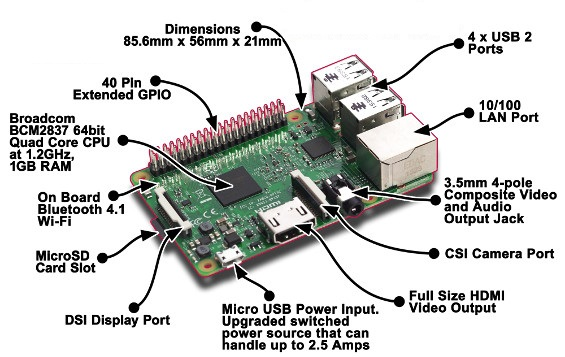
\includegraphics[width=1.0\textwidth]{rpi3}
	\caption[RaspberryPi V3.0]{Raspberry Pi Version 3.0}
	\label{fig:rpi3}
\end{figure}

\begin{landscape}
\begin{table}[htbp]
	\caption{}
	\begin{tabular}{|l|c|c|c|c|}
		\hline
		\multicolumn{1}{|c|}{\textbf{Modello}} & \textbf{Rpi} & \textbf{Rpi2} & \textbf{Rpi2 v1.2} & \textbf{Rpi3} \\ \hline
		Data di introduzione & 2014-07-01 & 2015-02-01 & 2016-10-01 & 2016-02-01 \\ \hline
		Processore SoC & Broadcom BCM2835 & Broadcom BCM2836 & \multicolumn{ 2}{c|}{Broadcom BCM2837} \\ \hline
		Architettura & ARMv6Z (32 bit) & ARMv7-A (32 bit) & \multicolumn{ 2}{c|}{ARMv8-A (32/64 bit)} \\ \hline
		CPU & ARM11 & ARM Cortex A7 & \multicolumn{ 2}{c|}{ARM Cortex A53} \\ \hline
		Numero di core & 1 & 4 & 4 & 4 \\ \hline
		Frequenza CPU (Mhz) & 700 & \multicolumn{ 2}{c|}{900} & 1200 \\ \hline
		GPU & \multicolumn{ 4}{c|}{Broadcom VideoCore IV} \\ \hline
		Memoria SDRAM & 512 & \multicolumn{ 3}{c|}{1024} \\ \hline
		Porte Usb 2.0 & 4 &  &  &  \\ \hline
		Input video & \multicolumn{ 4}{c|}{Connettore 15-pin MIPI  CSI usato con la Raspberry Pi camera} \\ \hline
		Output Video & \multicolumn{ 4}{l|}{HDMI (rev 1.3), video composito TRRS 3.5 jack, MIPI display interface DSI per pannelli LCD} \\ \hline
		Input Audio & \multicolumn{ 4}{c|}{su board attraverso porte I2S} \\ \hline
		Output Audio & \multicolumn{ 4}{c|}{analogico via jack 3.5mm, digitale via HDMI e su board I2S} \\ \hline
		Storage Slot & SD & \multicolumn{ 3}{c|}{MicroSDHC} \\ \hline
		Ethernet & \multicolumn{ 4}{c|}{10/100 Mbit/s} \\ \hline
		Wi-Fi & \multicolumn{ 3}{c|}{no} & 802.11n wireless \\ \hline
		Bluetooth & \multicolumn{ 3}{c|}{no} & Bluetooth 4.1 \\ \hline
		GPIO & \multicolumn{ 4}{c|}{17× GPIO plus the same specific functions, and HAT ID bus } \\ \hline
		Alimentazione & 600mA (3.0W) & \multicolumn{ 3}{c|}{800 mA(4.0 W)} \\ \hline
		dimensione & \multicolumn{ 4}{c|}{85.60 mm × 56.5 mm } \\ \hline
		Peso  & \multicolumn{ 4}{c|}{45g} \\ \hline
	\end{tabular}
	\label{}
\end{table}

\end{landscape}




La scelta per il progetto oggetto di questa tesi è stata per la versione 3  perchè mette a disposizione una potenza di calcolo superiorie a qualunche altro modello di RPi, grazie SoC BCM2837 all'interno del quale c'è  un 1Gb memoria, una CPU un quad-core ARM Cortex A53 a 64 bit a 1.2 Ghz ed una GPU VideoCore IV a 400Mhz, inoltre la Rpi3 è dotata del chip BCM43438 che fornisce connessione Wifi b/g/n e Bluetooth eliminando la necessità di utilizzare  un adatattore Wifi USB come avveniva nelle versioni precedenti.
L'antenna usata per le comunicazioni wireless si  trova sul bordo esterno della scheda, fuori dalla portata di possibili interferenze causate  da eventuali dispositivi e componenti aggiuntivi. L'integrazione delle comunicazioni wireless è una caratteristica importante se si vuole valutare l'aspetto di risparmio economico per una piattaforma IoT.

La Rpi ha quattro porte USB e una porta Ethernet 10/100 che condividono lo stesso bus gestito dal chip LAN9514. Questa soluzione può essere criticata  perchè non permette di sfruttare il 1Gbit sulla porta Ethernet, ma ai fini del nostro progetto non è un difetto che penalizza.


Nel dispositivo non è presente nessun tipo di memoria di massa, ma è presente un lettore di memorie MicroSD.
L'avvio del sistema avviene dalla scheda MicroSD all'interno della quale c'è una partizione con sopra il firmware, kernel e la configurazione del sistema.
Questo calcolatore è stato progettato per funzionare su diversi sistemi operativi Linux, RiscOS e Windows Core Iot.
Nell'appendice A descrivo come installare la versione Linux Raspian, il sistema operativo scelto per questo progetto.

\subsection{GPIO}
Tutte le versioni di questo computer hanno la possabilità di poter utilizzare GPIO  le GPIO sono delle porte che è possibile interagirgi
\begin{figure}[htbp!] 
	\centering    
	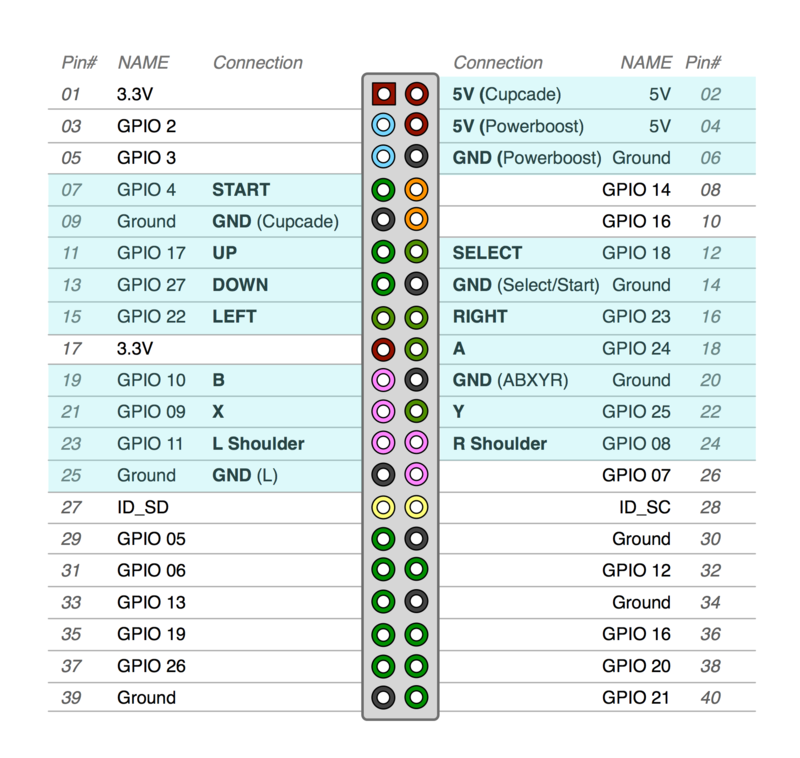
\includegraphics[width=1.0\textwidth]{gpio-map}
	\caption[Mappa GPIO]{La mappa delle Pin GPIO su Raspberry Pi}
	\label{fig:gpio-map}
\end{figure}
Nell'appendice B descrivo un semplice progetto che utilizza le porte GPIO

\subsection{Raspberry Camera}
Questa camera si collega a Raspberry Pi tramite la porta CSI e consente di creare video HD e scattare fotografie digitali,ha integrato il sensore di immagine CMOS IMX219PQ Sony da 8 megapixel ad alta qualità ed elevata sensibilità, con funzioni di video imaging ad alta velocità e supporto delle modalità video 1080p30, 720p60 e VGA90
\begin{figure}[htbp!] 
	\centering    
	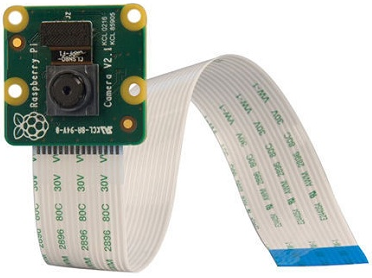
\includegraphics[width=1.0\textwidth]{camera}
	\caption[Raspberry Camera]{La Raspberry Camera}
	\label{fig:camera}
\end{figure}
Nell'appendice B descrivo come utilizzare i comandi offerti da raspian per utilizzare la raspberry camera

\subsection{L298N Motor Controller}
Si tratta di un modulo elettronico basato appunto sull’integrato L298, e sarà utilizzato per pilotare motori.
\begin{figure}[htbp!] 
	\centering    
	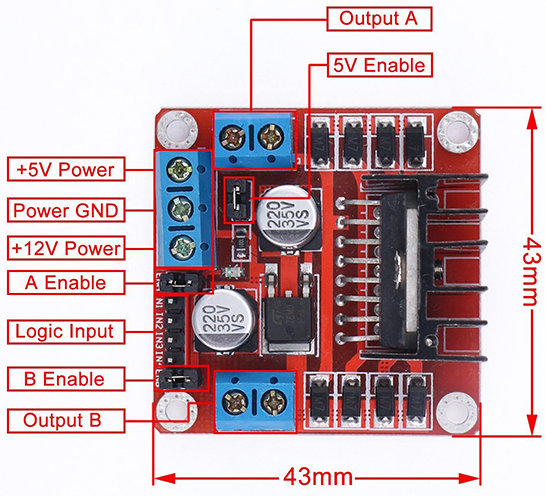
\includegraphics[width=1.0\textwidth]{L298N}
	\caption[L298N Motor Controller]{L298N Motor Controller}
	\label{fig:L298N}
\end{figure}
Questo circuito è composto da due connettori laterali ai quali collegare i motori, e da connettori frontali dove collegare l’alimentazione e le connessioni logiche atte a pilotare i carichi.
\begin{figure}[htbp!] 
	\centering    
	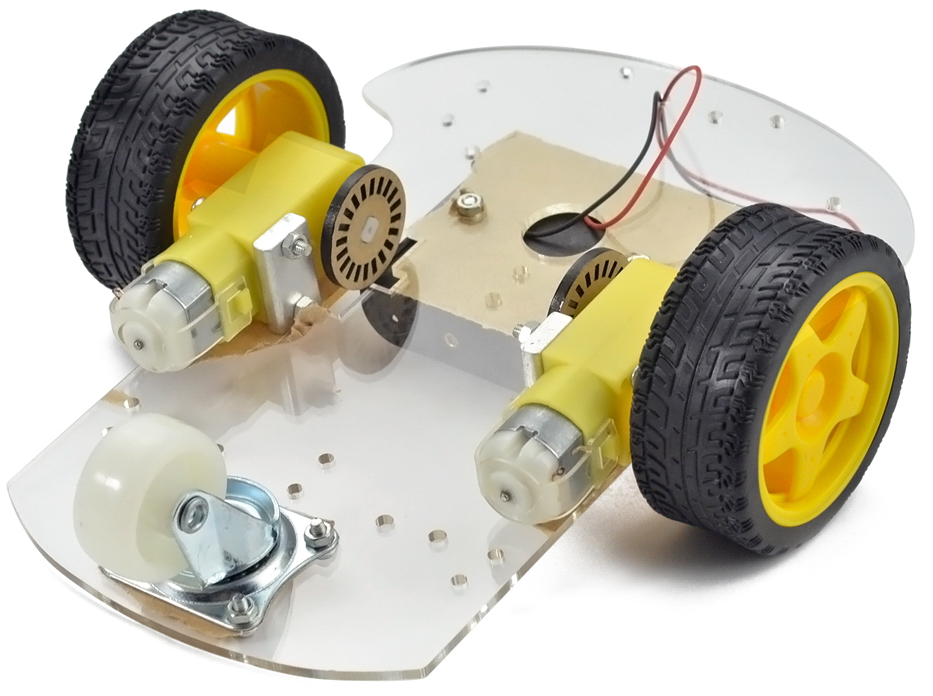
\includegraphics[width=1.0\textwidth]{chassis}
	\caption[Rover Chassis]{Rover Chassis con ruote, vano batteria}
	\label{fig:chassis}
\end{figure}
Questo modulo sarà collegato nel progetto finale direttamente allo chassis dove saranno presenti i motori e il vano batteria


\subsection{HC-SR04}
Il  sensore ad ultrasuoni hc-sr04 emette un impulso ad ultrasuoni e calcola il tempo impiegato dall’impulso per raggiungere il primo ostacolo di fronte a lui e tornare in dietro.
\begin{figure}[htbp!] 
	\centering    
	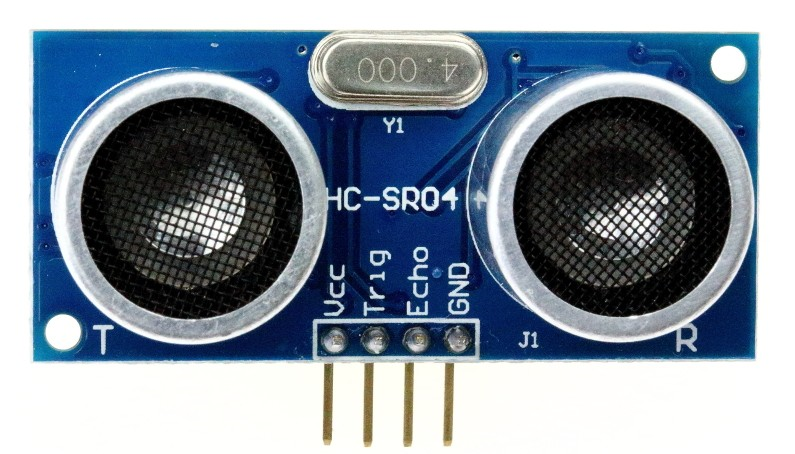
\includegraphics[width=1.0\textwidth]{hc-sr04}
	\caption[HC-SR04]{Il sensore ad ultrasuoni hc-sr04}
	\label{fig:hc-sr04}
\end{figure}
Il sensore dispone di 4 pin: Vcc (+5V), Trigger, Echo, GND. Si invia un impulso alto sul pin Trigger per almeno 10 microsecondi, a questo punto il sensore invierà il ping sonoro e aspetterà il ritorno delle onde riflesse, il sensore risponderà sul pin Echo con un impulso alto della durata corrispondente a quella di viaggio delle onde sonore, dopo 38 millisecondi si considera che non sia stato incontrato alcun ostacolo. Per sicurezza si aspettano in genere 50-60 millisec per far si che non vi siano interferenze con la misura successiva.


\subsection{BreadBoard}
Una breadboard permette di riprodurre il comportamento di un circuito stampato e non richiede saltatura di componenti, è possibile semplicemente inserire i componenti nei fori predisposti sulla board.
\begin{figure}[htbp!] 
	\centering    
	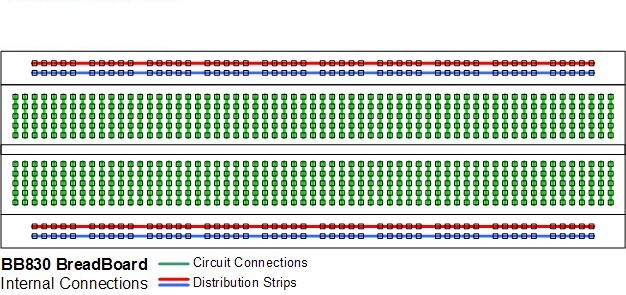
\includegraphics[width=1.0\textwidth]{breadboard}
	\caption[Breadboard]{Breadboard}
	\label{fig:breadboard}
\end{figure}
La breadboard che ho utilizzato è del tipo 830 fori in questo tipo di board ha due linee di punti laterali che corrono per tutta la lunghezza della breadboard e ogni punto di ogni singola linea è collegato tra di loro e solitamente queste linee vengo utilizzate per l’alimentazione. 
Le linee di punti interne della breadboard invece sono collegati a gruppi di due . i gruppi sono divisi da una scanalatura e ognuno dei quali è composto da 5 punti collegati tra loro.
Tutti i punti della breadboard che hanno una distanza di 2.54mm tra loro sono contrassegnati da un numero o da una lettera per facilitarne l'utilizzo.

Per facilitare la costruzione e il testing utilizzero un cavo piatto a 40 pin che collego dal Rpi3 ad un  t-cobbler sopra la breadboard , in questo modo posso lavorare con i GPIO di Rpi3 direttamente sulla board di testing
 

\begin{figure}[htbp!] 
	\centering    
	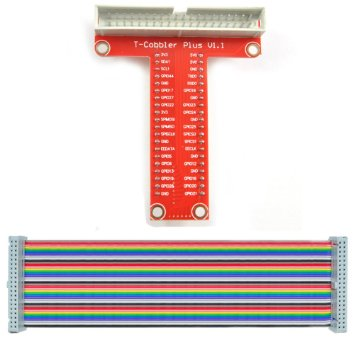
\includegraphics[width=1.0\textwidth]{t-cobbler-40}
	\caption[t-cobbler-40]{Cavo 40 Pin e T-Cobbler}
	\label{fig:t-cobbler-40}
\end{figure}

\section{Mono}
Mono è un progetto opensource coordinato da Xamarin, dal 2015 è diventata un'azienda sussidiaria di Microsoft, che ha lo scopo di realizzare  un insieme di strumenti compatibili con il Framework .NET di Microsoft ed aderenti allo standard Ecma anche per ambienti non Windows.
Il progetto mono implementa sia macchine virtuali chiamata Common Language Runtime per l'esecuzione dei programmi .NET per diverse piattaforme che compilatori per diversi linguaggi di programmazione.

Tra le CLR implementate c'è anche quella per Linux per processori x64 ARM e tra i compilatori di linguaggi implemetanti da Mono c'è sia il compilatore per \texttt{C\#} che quello per \texttt{F\#} che verrano utilizzati in questo progetto.

Nell'appendice C sarà  descritto come installare Mono e il compilatore \texttt{F\#} su Rpi3.

\section{\texttt{Raspberry\# IO}}
Nel progetto utilizzerò Raspberry# IO, è una libreria che consente di utilizzare le funzionalità GPIO di raspberry Pi su ambiente .NET/Mono, questa libreria è utilizzabile su linguaggio F#.
Nello specifico utilizzerò il package Raspberry.IO.GeneralPurpose che consente di utilizzare i Pin GPIO.
Questo package supporta le seguenti caratteristiche
Basso livello:

Accesso ai PIN GPIO attraverso 3 modalità: 
semplice (con uso di file), 
attraverso memoria, e 
completa (memoria attraverso "pseudo-interrupt"). Di default questa è modalità usata.
	Indirizzamento con il numero pin o con il numero di connettore pin
	Assegnamento dei Pin in base al modello e revisione del Raspberry Pi
	uso controllato delle risorse utilizzando un componente IDisposable e la capacità di utilizzare il rilevamento delle soglie , invece di polling
	Supporto al di sotto del millisecondo per il polling dei pin di input

Alto livello:
	Permette di personalizzare il nome dei Pin per consentire una maggiore leggibilità del codice
	Facilità di Uso, configurazione dichiarativa  dei Pin. Possibilità di ripristinare la polarità dei Pin (0/1). Permette di utilizzxare un pin in input come uno switch button.  
	Genera un evento quando lo status di un pin cambia , utlizzando il polling


\section{$ \texttt{ML}_{CoDa} $}
$ \texttt{ML}_{CoDa} $ è un linguaggio di programmazione orientanto al contesto. Questo linguaggio consente con alcuni costrutti di adattare il programma al contesto in cui viene eseguito. Il prototipo del linguaggio $ \texttt{ML}_{CoDa}} $ che userò è un estensione del linguaggio funzionale F#, della famiglia dei linguaggi ML.


Il contesto è l'ambiente dove le applicazioni vengono eseguite è un concetto fondamentale per il software adattivo. Il contesto può essere diviso in due parti: il contesto di sistema e il contesto applicativo.
Il contesto di sistema è la parte indipendente l'applicazione ad esempio l'hardware su cui viene esecutivo l'applicativo e l'ambiente fisico con il software può interagire.
il contesto applicativo è quello dipendente dall'applicazione come possono essere configurazioni utente.

Entrambi le parti in $ \texttt{ML}_{CoDa} $ sono rappresentati e gestiti in maniera omogenea. Questo linguaggio offre due componenti: una dichiarativa e una funzionale.

La componente dichiarativa  utilizza il DataLog per definire una base di conoscenza sulla quale i programmi adattivi possono interrogare il contesto e recuperare le informazioni che hanno bisogno.


L'appendice F descrivo la catena di compilazione di programma adattivo di esempio che utilizza $ \texttt{ML}_{CoDa} $ in modo da mostrare quali strumenti software sono utilizzati per questo progetto.


 
Nell'appendice D descrivo come testare gli esempi di $ \texttt{ML}_{CoDa} $ su Mono installato su Rpi3
 
Nell'appendice E implemento il progetto button-led in $ \texttt{ML}_{CoDa} $

\section{Node.js}

Node.js è un ambiente di esecuzione Javascript  opensource ed è disponibile su molte architetture, la piattaforma Node.js è basata sul Javascript Engine V8 di Google.
La principale caratteristica di Node.js è la sua  architettura event-driver per le I/O asincrone.
Inoltre offre anche un sistema di gestione dei pacchetti chiamato npm che permette di  in modo semplice e veloce di scaricare, installare e di integrare nel proprio progetto funzionalità aggiuntive offerte da moduli realizzati da una grandissima comunità.
Nel progetto utilizzero alcuni di questi pacchetti disponibili dal repository ufficale.


\subsection{Express.js}

\subsection{Telegram.js}
L’idea del progetto è di poter interagire con il robot con un I messaggistica, la scelta è caduta su telegram perché consente in maniera semplice di realizzare bot e interagirci attraverso API REST con risultanti in JSON. Nel repository Npm è presente il pacchetto Telegram.js che consente in modo semplice di integrare un applicazione node con le funzionalità offerte da telegram.

L'appendice E mostro come configurare Node.js per le funzionalità telegram

\section{Microsoft Cognitive Services} 
Cognitive Services (anche noto con il nome di Project Oxford) è un insieme di servizi esposti come API REST che permettono di aggiungere alle nostre applicazioni delle funzionalità “cognitive”, cioè funzionalità che abilitano le nostre applicazioni alla “comprensione” del mondo che le circonda.
Cognitive Services sfrutta la potenza del cloud e, in particolar modo, Azure Machine Learning per fornire una pletora di servizi che possiamo dividere nelle seguenti categorie:
•	Vision Service: sono quei servizi che permettono di analizzare immagini o video alla ricerca di informazioni. Fanno parte di questa categoria i servizi che ci consentono di individuare un volto o delle espressioni di un viso o le caratteristiche di un oggetto presente in un’immagine;



\chapter{Descrizione del Progetto}

% **************************** Define Graphics Path **************************
\ifpdf
    \graphicspath{{Chapter3/Figs/Raster/}{Chapter3/Figs/PDF/}{Chapter3/Figs/}}
\else
    \graphicspath{{Chapter3/Figs/Vector/}{Chapter3/Figs/}}
\fi

\section{Architettura Software}
 
 

\section{Realizzazione hardware}

\section{rpirover}
 
\section{rpiservice}

\section{fscrover}


%\include{Chapter4/chapter4}
%\include{Chapter5/chapter5}
%\include{Chapter6/chapter6}
%\include{Chapter7/chapter7}



% ********************************** Back Matter *******************************
% Backmatter should be commented out, if you are using appendices after References
%\backmatter

% ********************************** Bibliography ******************************
\begin{spacing}{0.9}

% To use the conventional natbib style referencing
% Bibliography style previews: http://nodonn.tipido.net/bibstyle.php
% Reference styles: http://sites.stat.psu.edu/~surajit/present/bib.htm

\bibliographystyle{apalike}
%\bibliographystyle{unsrt} % Use for unsorted references  
%\bibliographystyle{plainnat} % use this to have URLs listed in References
\cleardoublepage
\bibliography{References/references} % Path to your References.bib file


% If you would like to use BibLaTeX for your references, pass `custombib' as
% an option in the document class. The location of 'reference.bib' should be
% specified in the preamble.tex file in the custombib section.
% Comment out the lines related to natbib above and uncomment the following line.

%\printbibliography[heading=bibintoc, title={References}]


\end{spacing}

% ********************************** Appendices ********************************

\begin{appendices} % Using appendices environment for more functunality

% ******************************* Thesis Appendix A ****************************
\chapter{Configurazione SO Rover} 

\section{Raspian}

\subsection{Preperazione sdcard}
 
 

\subsection{Installazione Mono Framework}
 

\subsection{installazione Node.js}
 
\section{Installazione Fsharp}
 

% ******************************* Thesis Appendix B ********************************

\chapter{Installing the CUED class file}

\LaTeX.cls files can be accessed system-wide when they are placed in the
<texmf>/tex/latex directory, where <texmf> is the root directory of the user’s \TeX installation. On systems that have a local texmf tree (<texmflocal>), which
may be named ``texmf-local'' or ``localtexmf'', it may be advisable to install packages in <texmflocal>, rather than <texmf> as the contents of the former, unlike that of the latter, are preserved after the \LaTeX system is reinstalled and/or upgraded.

It is recommended that the user create a subdirectory <texmf>/tex/latex/CUED for all CUED related \LaTeX class and package files. On some \LaTeX systems, the directory look-up tables will need to be refreshed after making additions or deletions to the system files. For \TeX Live systems this is accomplished via executing ``texhash'' as root. MIK\TeX users can run ``initexmf -u'' to accomplish the same thing.

Users not willing or able to install the files system-wide can install them in their personal directories, but will then have to provide the path (full or relative) in addition to the filename when referring to them in \LaTeX.



\end{appendices}

% *************************************** Index ********************************
\printthesisindex % If index is present

\end{document}
